\label{sec:drahtlosedatenübertragung}
Drahtlose Datenübertragungverfahren ermöglichen die Übertragung von Informationen ohne elektrische Leiter. Sie nutzen elektromagnetische Wellen, Magenetfelder und elektrische Felder als Übertragungsmedium und können somit eine Kommunikation über Entfernungen von mehreren Kilometern oder mehr erreichen. 

Dieses grundlegende Prinzip ermöglicht verschiedene Anwendungen, die deutlich portabler und flexibler sind als kabelgebundene Verbindungen. Der Kernmechanismus besteht darin, die am Sender als elektrisches Signal vorliegenden Daten in elektromagnetische Wellen umzuwandeln, die sich durch die Umgebung ausbreiten können. Diese Signale können beim Empfänger wiederum in elektrische Signale umgewandelt und interpretiert werden. 

Für die drahtlose kommunikation werden überweigend elektromagnetische Wellen, insbesondere Funkwellen, eingesetzt. Drahtlose Kommunikationssysteme arbeiten in verschiedenen Frequenzbändern, die stark reguliert sind, um mögliche Interferenzen zu vermeiden \autocite{GrundkenntnisseDrahtlosenKommunikation2023}.

Bekannte Modulationsverfahren lassen sich in Analoge und Digitale Verfahren aufteilen. Analoge Modulation verändert die Parameter des Trägersignals, bei der Amplitudenmodulation wird die Amplitude und bei der Frequenzmodulation die Frequenz kontinuierlich entsprechend dem analogen Eingangssignal angepasst. Bei der digitalen Modulation hingegen wird zwischen diskreten, fest definierten Zuständen umgeschaltet, um digitale Daten zu übertragen. \autocite[S. 112 ff.]{ziemerPrinciplesCommunicationsSystems2015} \autocite[S. 156 ff.]{ziemerPrinciplesCommunicationsSystems2015}

Ein einfaches Digitales Übertragungsprotokoll ist hier bei das Frequency Shift Keying (FSK), dabei werden digiale informationen durch die Variation der Frequenzen eines Trrägers kodiert. Im Wesentlichen wird die Trägerfrequenz periodisch zwischen mehreren Frequenzen verschoben, wobei jede Frequenz ein bestimmtes digitales Symbol darstellt.

Das einfachste FSK-Verfahren ist die binäre FSK (Binary FSK, BFSK oder 2-FSK), bei der zwei unterschiedliche Frequenzen verwendet werden, um die Binärziffern "`0"' und "`1"' zu repräsentieren. Eine höhere Frequenz repräsentiert eine binäre "`1"', während eine niedrigere Frequenz eine binäre "`0"' darstellt, wie in Abbildung \ref{fig:frequency-shift-keying} gezeigt. Wenn die zu übertragenden Daten eine "`0"' enthalten, wird die Trägerfrequenz $t_1$ verwendet um dieses Bit zu übertragen, wenn die Daten eine "`1"' sind, wird die Trägerfrequenz $t_2$ verwendet.\autocite{FrequencyShiftKeyingModulation2024}

\begin{figure}[H]
\centering
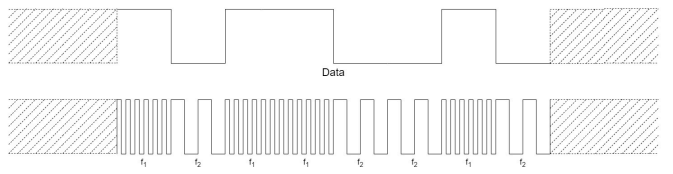
\includegraphics[scale=.5]{figures/asstes/frequency-shift-keying.png}
\caption{Frequency Shift Keying \autocite {FrequencyShiftKeyingModulation2024}}
\label{fig:frequency-shift-keying}
\end{figure}